\documentclass[oneside,12pt]{memoir}
\def\mychaplineone{Developer notes for}
\def\mychaplinetwo{ESGF Node Manager}
%\def\mychaplinethree{And Some More...}
\def\myauthone{Prashanth Dwarakanath}
\def\myauthtwo{Sasha Ames}
%\def\myauththree{Torgny Fax\'en}
\def\mypress{Earth System Grid Federation}
\usepackage{chengi}
\usepackage{biblatex}
\bibliography{thebib}
\DefineBibliographyStrings{english}{%
  bibliography = {References},
}
\def\nm{Node Manager{ }}
\def\vernum{December 5, 2014}
\setcounter{tocdepth}{2}
\thispagestyle{empty}
\titleGM
\chapterstyle{BlueBox}
\pagestyle{mystyle}
\begin{document}
\frontmatter
\hypertarget{mytocmarker}
\tableofcontents
\mainmatter
\setcounter{secnumdepth}{2}
\chapter{Solution Design}
\section{Overview}


\section{Design Considerations}
\begin{itemize}
\item 


We are interested in a hierarchical framework for node management rather than a pure p2p.  In this case nodes elect "super-nodes" that perform additional tasks than "member-nodes".  Our goal for scalability is to have a balance of super vs member nodes to ensure that no super-node becomes oversubscribed.  Super-nodes operate at the "project" level.   
\item
A node that serves as the "super-node" for project A can be a member node for project B.  Super-nodes can serve in that role for multiple projects.    Configuring a node for eligibility for selection to become a super node is voluntary, but important for the federation to have an "adequate" number of candidates.
\item
Vetting for a super node. Hand-picked initial super-nodes.  
\item
Member nodes pass messages.  
\item
Node manager admin interface.  Allow admins to eg. sign certs, vet nodes,  
\item
Tree-based communication between super nodes and member nodes to reduce communication overheads, ie. avoid $n^2$ patterns.  We expect a ``wide'' tree with ``few" hops. Or consider filled-out binary tree structure (see below). 
\item 
Need to maintain backward compatibility with format of registration.xml etc, to not break existing parsers. 
\end{itemize}


\section{Breakup of tasks}

\subsection{Communication}

\begin{enumerate}
\item
Review AVL tree reorganization
\item
Model deterministic communication
\end{enumerate}


%\subsection{zookeeper evaluation}
%\begin{enumerate}
%\item
%Performance evaluation
%\item
%Evaluate functionality
%\item
%Assess  API
%\end{enumerate}

\subsection{metrics gathering}
\begin{enumerate}
\item Investigate logger issue
\item Decouple logger from Node Manager
\item Ensure generation of registration.xml
\end{enumerate}



\section{System Architecture}
\begin{center}
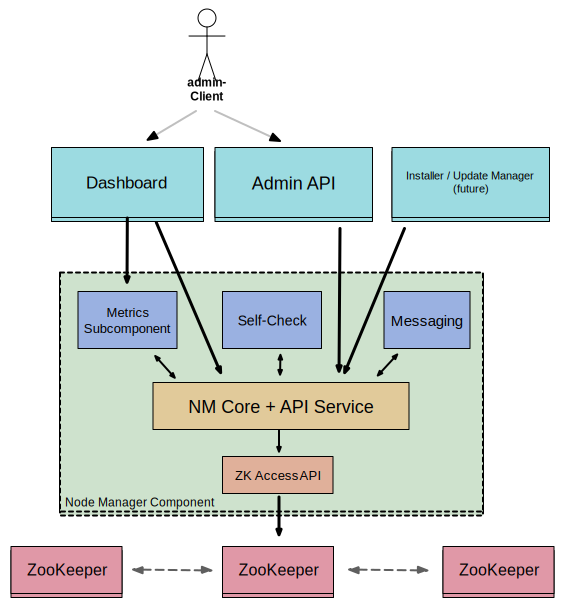
\includegraphics[width=5in]{presentation/NM-design.pdf}
\end{center}
\newpage

\subsection{Components}
These are the main components of the solution.
\begin{enumerate}
\item
\textbf{Local config file} 
\begin{enumerate}
\item Membership to projects.
\item Projects to serve as supernode/standby node (voluntary).



\end{enumerate}




%Apache ZooKeeper seems to be a very promising fit for this role, so this component shall henceforth simply be refered to as ZooKeeper.
%After looking at ZooKeeper, we opt against incorporating  ZK in the node manager/ esgf software stack.  Instead we focus on implementing a component that loosely model's its communication style on ZK.  

\item \textbf{Files in central git repository}
\begin{enumerate}
\item Project specific config parameters. ex: thredds\_exclude\_variable list
\item Comprehensive list of supernodes for membernodes to consult.
\item Global configuration parameters for supernodes: limits for number of members to serve etc
\end{enumerate}
\item \textbf{Node Manager Service}
\begin{enumerate}
\item Membernodes service status
\item Current list of supernodes and the membernodes they serve (node map).
\end{enumerate}

%A component that serves as a `feeder', to the zookeeper. This would also provide an administrative interface to the node manager. This is the component of the node manager that is meant to be exposed to the federation, and not the ZooKeeper itself, and it includes the ESGF Node Manager API. Henceforth, this component shall simply be refered to as the node manager. The node manager will also be used by local admins, to generate requests for federation membership or certificate signing and allow supernode admins to ratify/sign these requests. The node manager would also be responsible for collection of metrics.

\end{enumerate}

\subsection{Communication handler subcomponent}
Communication occurs via https client to the apache server listening on the nodes.   The apache service pushes messages back to local API.    We describe the communication use cases and patterns below.


\subsection{Metric subcomponent}

This subcomponent produces the metrics that appear on the dashboard or other UI.Much metric ``raw" data will be found in the log files.  A crawler procedure can gather stats from the logs.   The metric service can include aggregate information from the provenance collection system. \yellowline{Also, the currently built-in hooks to log realtime download activity etc would have to be refined to ensure greater accuracy and eliminate problems such as false positives/negatives.}
%An optional part of this is a centralized collection of the log data that can be queried efficiently.  We expect that this would be on data center supernodes.  

%Some metrics are based on node state managed by the "feeder" service.  The zookeeper DFS can be used as the metastore for metric metadata.  
\subsection{Self-check subcomponent}
This is a subcomponent of the node manager which is responsible for carrying out sanity checks at regular intervals, on itself. When it fails the sanity checks, it contacts the local node manager to flag itself ineligible to continue as a supernode/standby supernode/member node. When the node passes a subsequent sanity check, the self-check component contacts the local node manager, to flag itself ready for resumption of duties.  The self-check subcomponent would also use the messaging subcomponent, to send out alert notifications to the local admin, when sanity checks fail.

\subsection{Messaging subcomponent}
The messaging subcomponent is used by the self-check subcomponent, to alert the local admin, when the state of the node changes, i.e. fails a sanity check, or clears one, after having been flagged down by previous checks.



\section{Node manager capacities}
Each and every ESGF installation, irrespective of role, i.e. data, compute etc, would have the node manager as a component.  However, the node manager itself can function in different capacities. 
\begin{enumerate}
\item \textbf{Membernode}: This is the default capacity of a node manager. It cannot query other node manager instances and can only pass on validated messages. See Section~\ref{commcases} for more. A membernode can volunteer to be a supernode or a standby supernode.
\item \textbf{Supernode}: This is a membernode which volunteered to function as a supernode and was vetted Responsible for querying nodes which it is responsible for.  A federation would have multiple superposed which divide the workload among themselves. Supernodes also perform aggregation of gathered metrics. 
\item \textbf{Standby supernode}: A standby supernode is a membernode which volunteered to function as a supernode when the number of supernodes in the federation falls below a predefined threshold. These nodes temporarily function as supernodes and return to being standy supernodes, when the supernode count stabilizes in the federation.
\end{enumerate}

\section{Communication use-cases}
\label{commcases}
%A bulk of internode communication is handled implicitly by ZooKeeper, releasing us from having to explicitly establish communication for tasks such as leader election, but the ZooKeeper is not exposed to the outside world. Instead, it is controlled/accessed with the node manager, which serves as both a controller for ZooKeeper itself, and also as a wrapper for ZooKeeper. This would need node manager instances to communicate with each other. Let's consider the types of communication between node manager instances.



\begin{enumerate}
\item \textbf{Supernode to membernode}: metric queries, status queries, status change notifcation (standby to supernode, viceversa etc)
\item \textbf{Supernode to supernode}: Shoot the node in the head, in case of malfunction.  Shared information updates.  Peer checks.
\item \textbf{Membernode to membernode}: passing on authenticated messages received from supernodes.  This communication is TBD (could be tree based using same principe as used within tree network of super nodes. % (this is implicit in zookeeper's communication)  
\item \textbf{Membernode to supernode}: Pushing local config status etc.
\end{enumerate}

\begin{center}
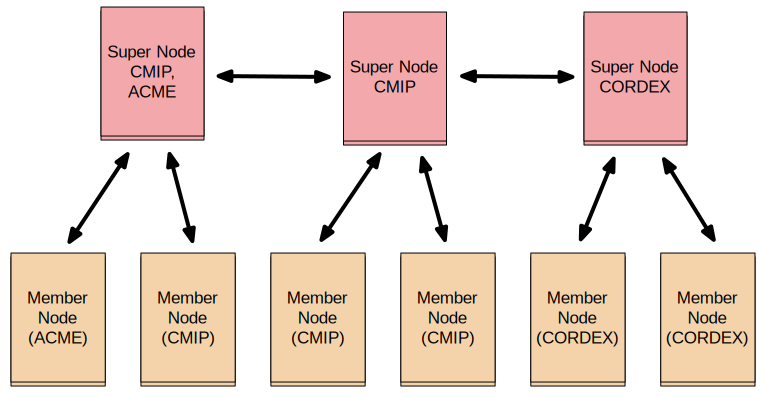
\includegraphics[width=5in]{presentation/ESG-node-org.pdf}
\end{center}

\section{System Design}

Tree-based node communication among SuperNodes.  Communication among peers is deterministic based on a node assigned number (taken from the master list of SuperNodes).   Leaf nodes have additional communication with their siblings to increase the number of checks, so all nodes can have 2-3 peers monitoring each at a time.  Standby nodes are assigned potential slots in the event they become activated so each know who the peers will be.  Standby nodes function as member nodes, so these nodes have been assigned a SuperNode and that SuperNode is independent of where the standby nodes will reside in a peer.  Member nodes are shown attached to node \# 8 in this example.  However all SuperNodes are expected to have some assigned member nodes, but not essential.  SuperNodes can still function in a relay role without any member nodes and may be needed to take on member nodes as soon as another fails or imbalance occurs. 

\begin{enumerate}
\item The comprehensive list of supernodes is manually updated in the controlling git repository, which also contains global configuration parameters for supernodes; ex: maximum number of membernodes that can be serviced by supernode etc
\item When a new node is brought up, it fetches the list of supernodes and starts communicating with each of them, in sequence, till it contacts a supernode that admits the member node. When a new node contacts a supernode for membership, these are the possible results:
\begin{enumerate}
\item \textbf{No response}: if supernode is down or unreachable.
\item \textbf{Deny}: if the contacted node is no longer operating as a supernode or if the supernode is already fully subscribed.
\item \textbf{Accept}: if the supernode agrees to serve it.
\end{enumerate}
\item super-nodes establish project group ZK-node directory instances.  Each project includes the min and max thresholds for super node count.  The threshold may increase if a larger number of project nodes join a group.  We expect that these settings will initially be controlled by a super-node administrator, but could be automated.


\item Super and Member nodes establish ephemeral nodes for project group membership.  Based on the property of ephemeral nodes, an instance will not persist if a creator Member Node becomes unavailable.  The ephemeral node instance contains the high-level characteristics for the node, such as the node types running (data, index, idp, compute),  maybe user, data set counts, other projects hosted.  
\item Standby nodes set their status in a subdirectory for the project group

\item the first standby node will assume super node responsibility if the project SN count threshold dips below the minimum allowed.  A thread in the node manager service may poll the ZK ephemeral nodes to see if the change over is required, then can invoke the SN role library functions.
\item SuperNode legacy service for registration.xml pulls node "alive" information to feed to the Dashboard.  

\end{enumerate}
\begin{center}
\includegraphics[width=5in]{presentation/Node-comm-v2.pdf}
\end{center}


\section{Authentication mechanisms}
Distinction to be made between user authentication and system authentication, as certain privileged operations may need to be executed without human intervention. This would need a system or process to be authorized to perform the operation. 

\section{Feedback and questions from the F2F 2014}
\begin{enumerate}
\item Can ZooKeeper be proxied on http/https, to avoid having to open up further ports.
\item Can the \nm implement federated attribute service?
\item Luca's virtual organization management vs project level management by \nm How do they fit in ?
\end{enumerate}


\section{Issues and questions}
This is to be a place to list out problems that need to be handled.
\begin{enumerate}
\item
Do we use zookeeper?
\begin{enumerate}
\item \redline{Implementing dynamic changes by adding or removing ZKs might be problematic.}
\item \redline{ZK seems to be designed to operate behind a firewall, preferably with all hosts on the same subnet.}
\item \redline{ZK not designed with focus on security, as common implementations are cluster management etc, all behind firewall}
\item \redline{Getting hosts to open up additional ports is cumbersome and a backward step} 
\end{enumerate}
\item
To what extent can we rely if we do,  what do we need to implement for the \nm?
\item

Is zookeeper a fit for management?
\item
Can zookeeper manage group-level access control?  We think it can.  Need to evaluate.
\item
Is zookeeper python API adequate?

\item
Deal with "spoofed" node; ensure relayed information is legitimate. 
\item
%Need to choose centralized query service database system.  Use Hadoop, spark, Hive, Cassandra, or some RDBMS?
Need the supernode to query nodes for metrics and perform aggregation where necessary.

\end{enumerate}
\section{To revisit}
\begin{enumerate}
\item Support for automated replication of datasets
\item Support for an update manager service (to supplant present esgf-installer)
\item Metrics collection: what needs to be done for aggregation? Does it clash with what Sandro intends to do?
\end{enumerate}
%\nocite{KandR}
\printbibliography
\hypertarget{mymarker}{}
\printindex
\end{document}
